\chapter{Systembeskrivelse}
\section{Systemoversigt}

	\begin{figure}[h!]
		\centering
		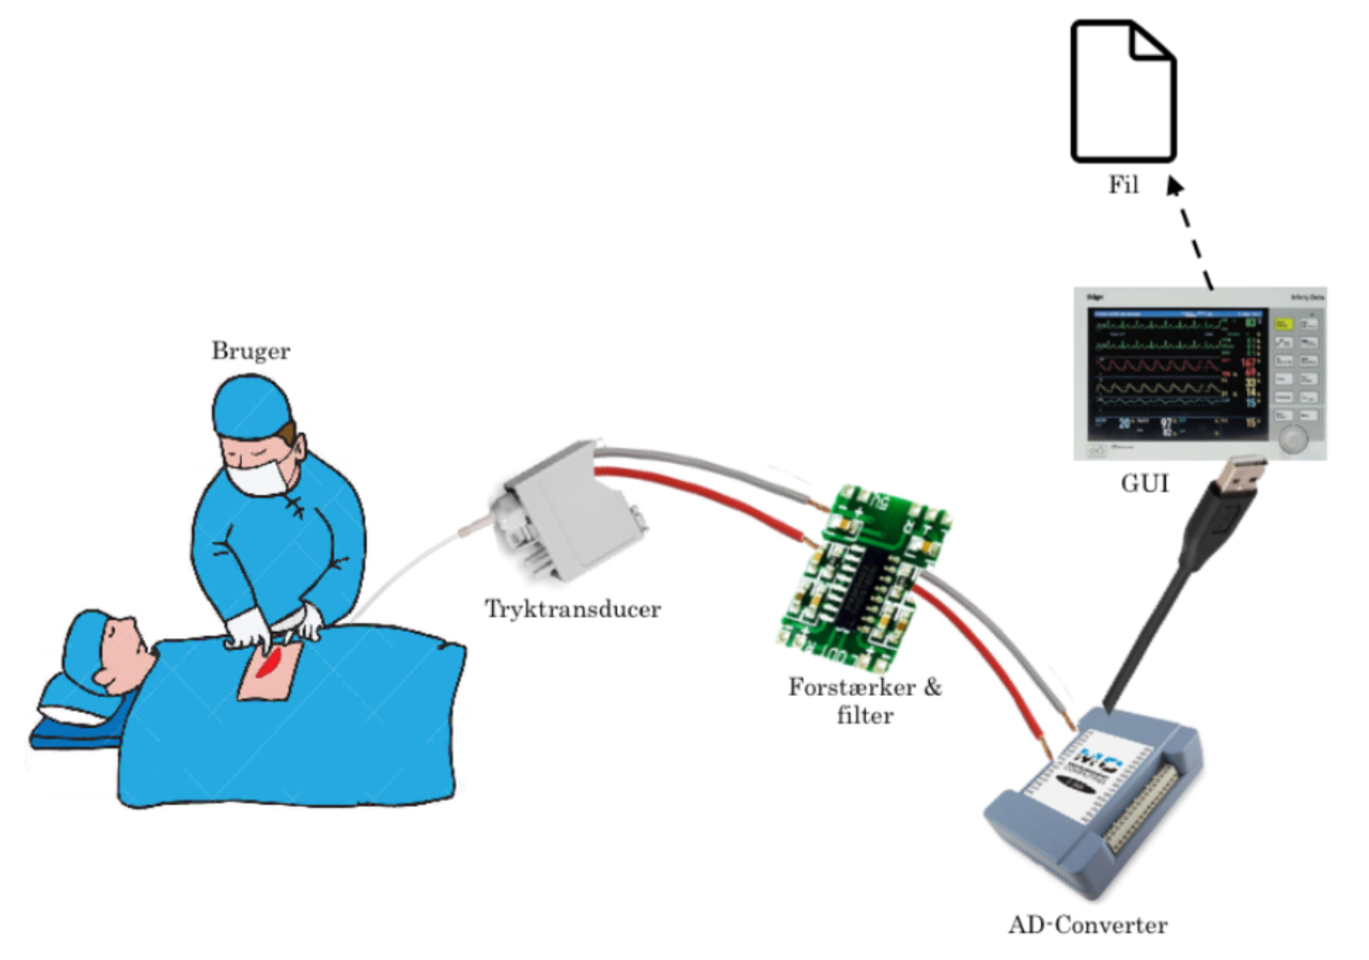
\includegraphics[width=0.55\linewidth]{Systembeskrivelse/Systemoversigt}
		\caption{Systemoversigt}
		\label{fig:Systemoversigt}
	\end{figure}
\vspace{1 cm}

\section{Systembeskrivelse}
På figur \ref{fig:Systemoversigt} ses systemoversigten for vores blodtrykmålesystem, der har til formål at kunne måle og vise en patients blodtryk og puls på en brugergrænseflade. 

Systemet består af:

\begin{itemize}
	\item Tryktransducer
	\item Forstærker
	\item Subtraktor
	\item Anti-aliaseringsfilter
	\item AD-Converter (NI DAQ 6009 USB)
	\item Computer
	\item Bluetooth højtaler
	\item Skærm
	\item Brugergrænseflade	
\end{itemize}

Brugergrænsefladen er bygget op som et Graphical User Interface (GUI) hvorpå det målte blodtryk visualiseres kontinuert i form af en graf. Det systoliske-, diastoliske-, median blodtryk og puls vises i form af tal. Brugergrænsefladen består af knapper, der har forskellige funktioner. For nærmere beskrivelse af brugergrænsefladens funktioner henvises der til dokumentet kravsspecifikation. \clearpage

\subsection{Alarmer}
Systemet skal i henhold til standard 60601-1-8 vedrørende alarmering kunne alarmere ved eventuelle fejl eller ændringer. I forhold til brugssituationen af blodtrykmålesystemet vurderes det at systemet skal kunne alarmere, når der er fald eller stigning i blodtryk eller puls uden for de justérbare grænseværdier.
Alarmen er en high priority, som alarmerer visuelt og auditivt. For krav til alarmen henvises til dokumentet kravspecifikation afsnit 1.12 og dokumentet for alarmspecifikationerne, som er udarbejdet ud fra standard ISO 60601-1-8: 2017.


\clearpage 